%---------------------------------------------------------------------------
%   PACKAGES AND OTHER DOCUMENT CONFIGURATIONS
%---------------------------------------------------------------------------
\documentclass[final]{beamer}
\usepackage{gensymb}
\usepackage{textcomp}
\usepackage[scale=1.24]{beamerposter} % Use the beamerposter package for laying out the poster
\usetheme{confposter} % Use the confposter theme supplied with this template
\setbeamercolor{block title}{fg=purple,bg=white} % Colors of the block titles
\setbeamercolor{block body}{fg=black,bg=white} % Colors of the body of blocks
\setbeamercolor{block alerted title}{fg=white,bg=white} % Colors of the highlighted block titles
\setbeamercolor{block alerted body}{fg=black,bg=white!10} % Colors of the body of highlighted blocks
% Many more colors are available for use in beamerthemeconfposter.sty
%---------------------------------------------------------------------------
% Define the column widths and overall poster size
% To set effective sepwid, onecolwid and twocolwid values, first choose how many columns you want and how much separation you want between columns
% In this template, the separation width chosen is 0.024 of the paper width and a 4-column layout
% onecolwid should therefore be (1-(# of columns+1)*sepwid)/# of columns e.g. (1-(4+1)*0.024)/4 = 0.22
% Set twocolwid to be (2*onecolwid)+sepwid = 0.464
% Set threecolwid to be (3*onecolwid)+2*sepwid = 0.708
\newlength{\sepwid}
\newlength{\onecolwid}
\newlength{\twocolwid}
\newlength{\threecolwid}
\setlength{\paperwidth}{48in} % A0 width: 46.8in
\setlength{\paperheight}{38.4in} % A0 height: 33.1in
\setlength{\sepwid}{0.024\paperwidth} % Separation width (white space) between columns
\setlength{\onecolwid}{0.22\paperwidth} % Width of one column
\setlength{\twocolwid}{0.464\paperwidth} % Width of two columns
\setlength{\threecolwid}{0.708\paperwidth} % Width of three columns
\setlength{\topmargin}{-0.75in} % Reduce the top margin size
%---------------------------------------------------------------------------
\usepackage{graphicx}  % Required for including images
\usepackage{booktabs} % Top and bottom rules for tables
\graphicspath{{../plots/}}
%---------------------------------------------------------------------------
%   TITLE SECTION 
%---------------------------------------------------------------------------
\title{Measuring $^{nat}$La(p,x) Cross Sections from 35-60 MeV by Stacked Foil Activation} % Poster title
\author{$^1$Jonathan Morrell$^*$, $^1$Andrew Voyles, $^{1,2}$Lee Bernstein, $^2$Shamsuzzoha Basunia} % Author(s)
\institute{1: Nuclear Engineering, University of California, Berkeley\\
2: Lawrence Berkeley National Laboratory
} % Institution(s)
%----------------------------------------------------------------------------
\begin{document}
\addtobeamertemplate{headline}{} 
{\begin{tikzpicture}[remember picture,overlay] 
\node [shift={(-10cm,-11.0cm)}] at (current page.north east) {
\includegraphics[height=7cm]{photos/Berkeley_Lab_Logo_Large.png}}; 
\end{tikzpicture}
%\begin{tikzpicture}[remember picture,overlay] 
%\node [shift={(-27cm,-10.5cm)}] at (current page.north east) {
\includegraphics[height=7cm]{photos/primarylogo.png}}; 
%\end{tikzpicture}
\begin{tikzpicture}[remember picture,overlay] 
\node [shift={(-100.5cm,-12.0cm)}] at (current page.north east) {
\includegraphics[height=4.5cm]{photos/NE_Logo.png}}; 
\end{tikzpicture}
}
\begin{frame}[t] % The whole poster is enclosed in one beamer frame
\begin{columns}[t] % The whole poster consists of three major columns, the second of which is split into two columns twice - the [t] option aligns each column's content to the top
\begin{column}{\sepwid}\end{column} % Empty spacer column
\begin{column}{\onecolwid} % The first column
%----------------------------------------------------------------------------
%   LEFT
%---------------------------------------------------------------------------
\begin{block}{Introduction}
\small{\hspace*{50pt}Proton induced nuclear reactions in the tens of MeV range can be used for the production of radioactive isotopes with minimal contaminants, which makes them a compelling production mechanism for medical diagnostic and therapeudic isotopes \cite{TARKANYI2016262}.  Nuclear data for many of these reactions is scarce, and yet is critical for researchers wishing to optimize irradiation parameters for the production of these radioisotopes \cite{nuclear_data_needs}.
}

\begin{figure}
\fbox{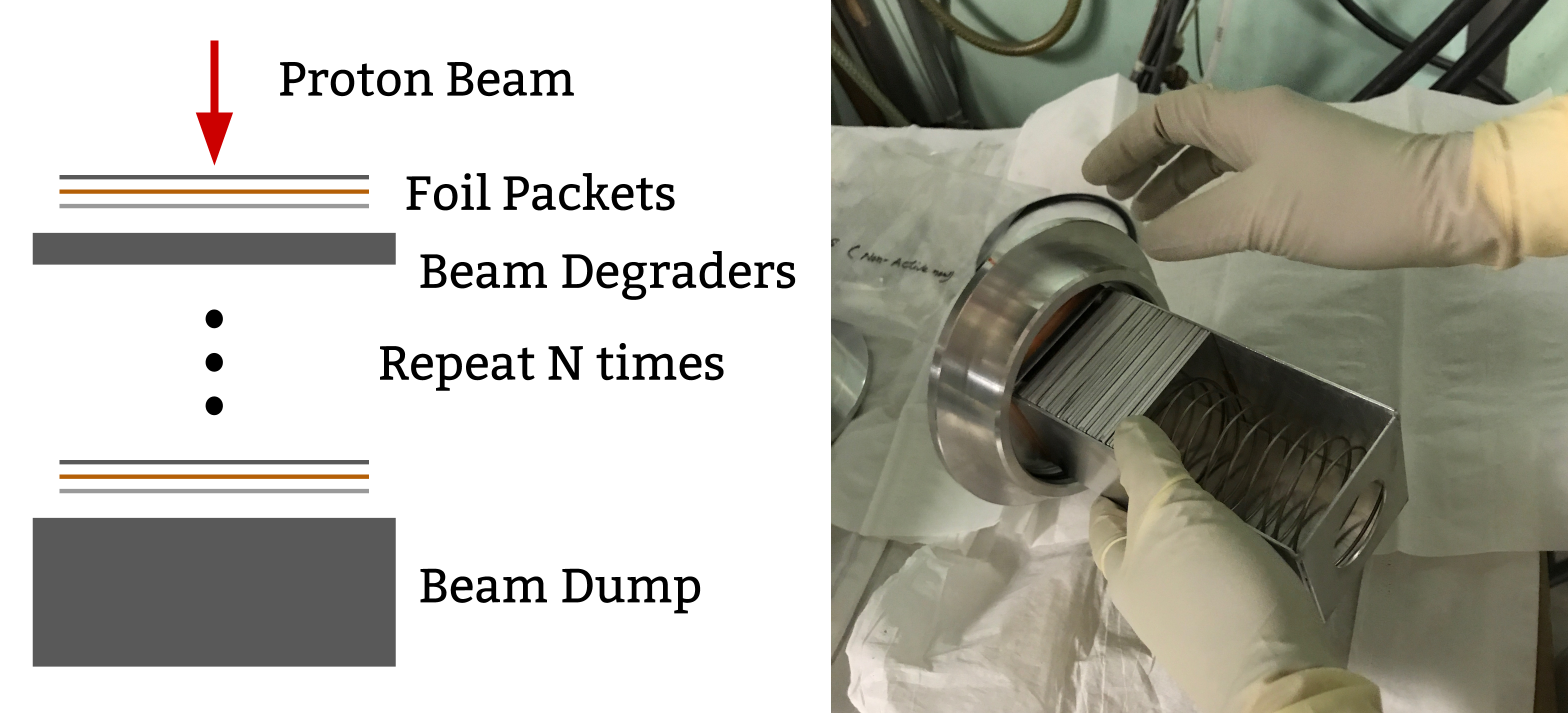
\includegraphics[width=0.8\linewidth]{photos/schematic_stack.png}}
\caption{Schematic of the foil stack (left) and photograph of stack prior to irradiation (right).}
\end{figure}

\small{\hspace*{50pt}In this experiment, we measure the $^{nat}$La(p,x) reaction cross sections with a particular interest in the (p,6n) reaction on $^{139}$La (99.9119\% n.a.) \cite{ensdf} for the production of $^{134}$Ce, an isotope with applications as a positron emitting analogue of $^{225}$Ac.  $^{225}$Ac is a promising therapeudic isotope, however because it has no $\beta^+$ emissions a chemical analogue such as Ce must be used to study it's bio-kinetics.  Data from this experiment is also important to nuclear reaction modelling.  Pre-eqillibrium reactions and spin-state distributions influence the cross sections for these reactions, and measuring these cross sections using the stacked foil method will be meaningful to the reaction modelling community.

%\hspace*{50pt}In a stacked foil activation experiment one can measure a reaction cross section by measuring the activity induced in a thin foil of known areal number density by a beam of known intensity.  Many such foils can be placed one in front of another to form a "stack", and the cross section can be measured at many different energies by characterizing the energy loss within the stack.
%
%\hspace{50pt}The foil activities induced by the proton reactions were measured by detecting $\gamma$-ray emissions using a high-purity Germanium (HPGe) detector.  An example of a $\gamma$-ray spectrum collected in this experiment is shown in Fig. 2.  The beam current was measured using "monitor" foils, which have well characterized charged particle cross sections, and typically produce long-lived radionuclides with intense $\gamma$-ray emission lines.

\hspace{50pt}Measurement of these reaction cross sections can be broken down into a number of discrete steps:

\begin{itemize}
\item Calibrate the HPGe $\gamma$-ray detector
\item Measure the mass and dimensions of the target foils
\item Assemble the stack and secure in the beamline
\item Irradiate for fixed duration and proton current
\item Count irradiated foils with HPGe detector
\item Fit peaks in the monitor and target foil spectra (Fig. 2)
\item Determine end-of-beam foil activities ($A_0$)
\item Determine beam current and energies
\item Calculate cross-sections
\item Compare results to EXFOR, TALYS and EMPIRE
\end{itemize}

}
\begin{figure}
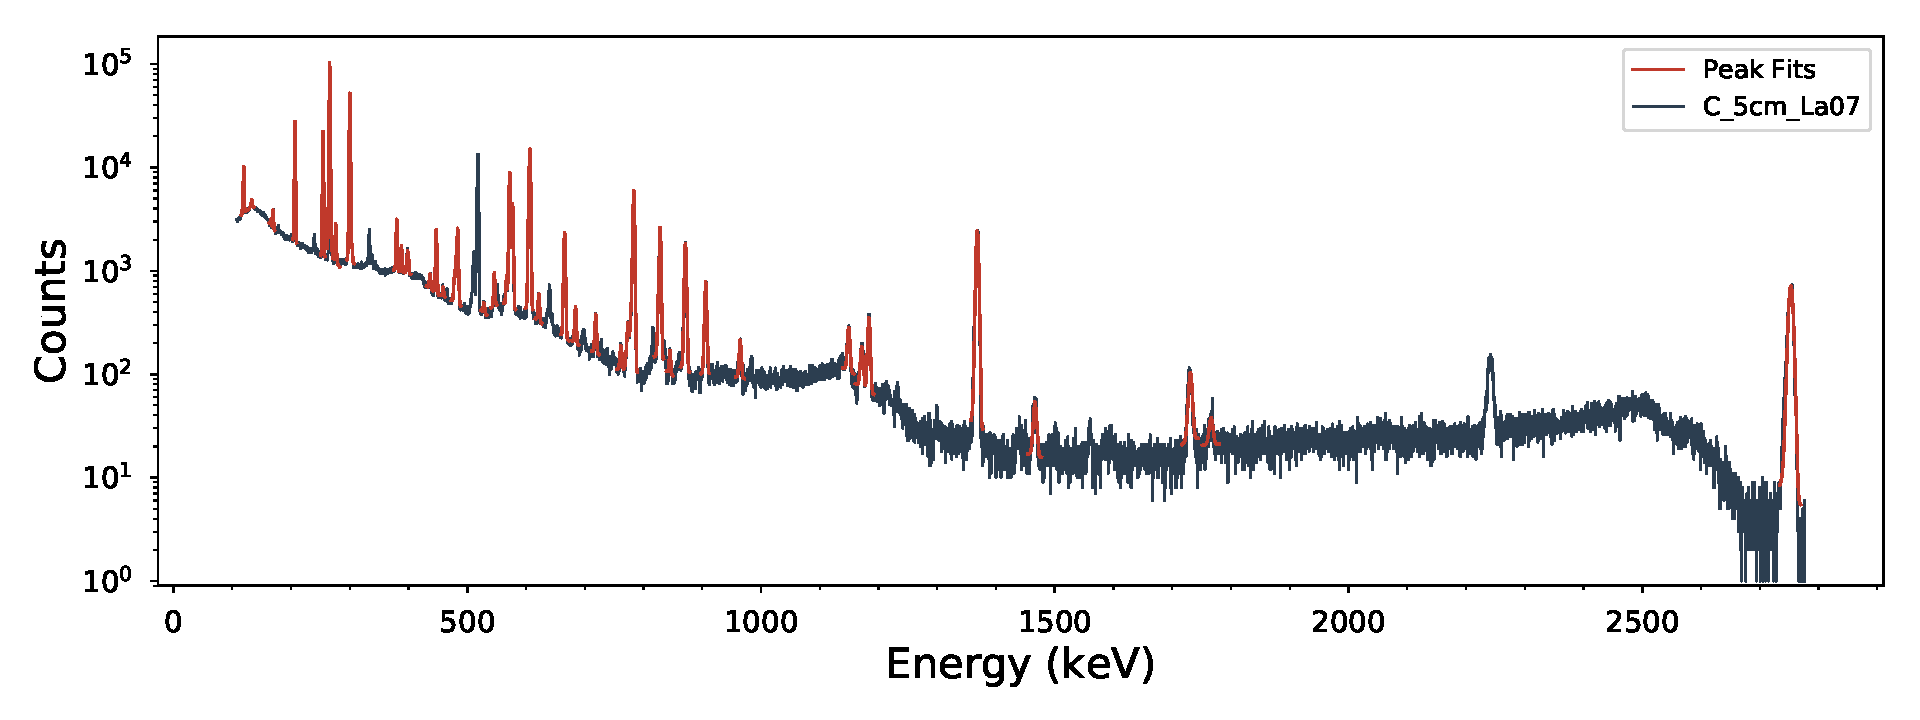
\includegraphics[width=0.9\linewidth]{peak_fits/C_5cm_La07_fits.pdf}
\caption{Example of $\gamma$-ray spectrum from the 7$^{th}$ lanthanum foil, with peak fits indicated in red.}
\end{figure}

\end{block}
%----------------------------------------------------------------------------
\end{column} % End of the first column
\begin{column}{\sepwid}\end{column} % Empty spacer column
\begin{column}{\twocolwid} % Begin a column which is two columns wide (column 2)
%----------------------------------------------------------------------------
%        MIDDLE
%----------------------------------------------------------------------------

\begin{figure}
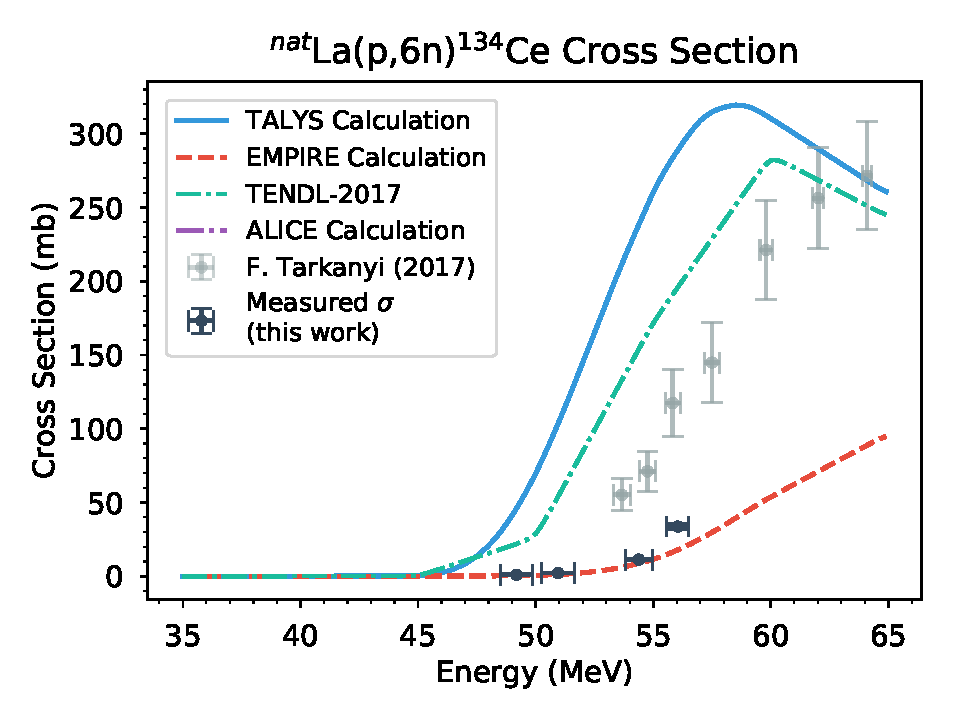
\includegraphics[width=0.32\linewidth]{cross_sections/134CE.pdf}
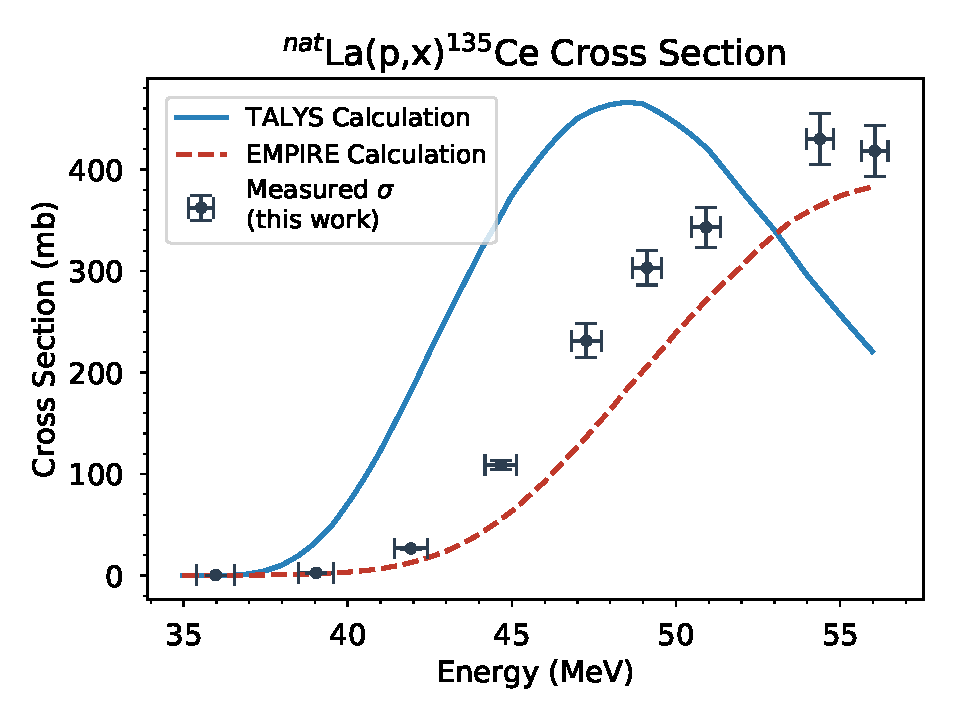
\includegraphics[width=0.32\linewidth]{cross_sections/135CE.pdf}
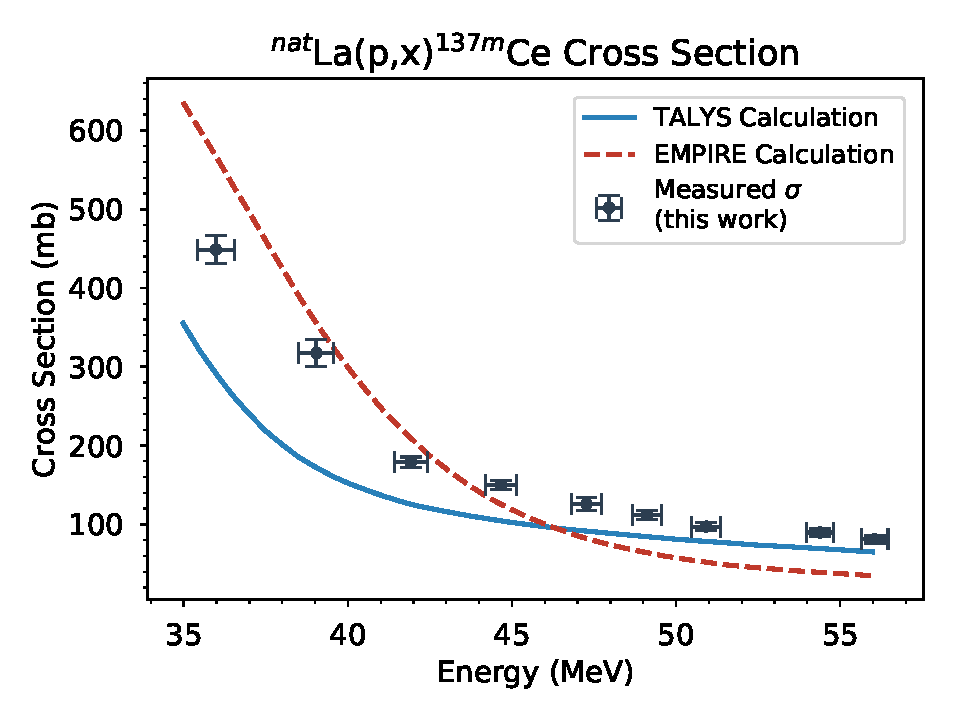
\includegraphics[width=0.32\linewidth]{cross_sections/137CEm.pdf}\\
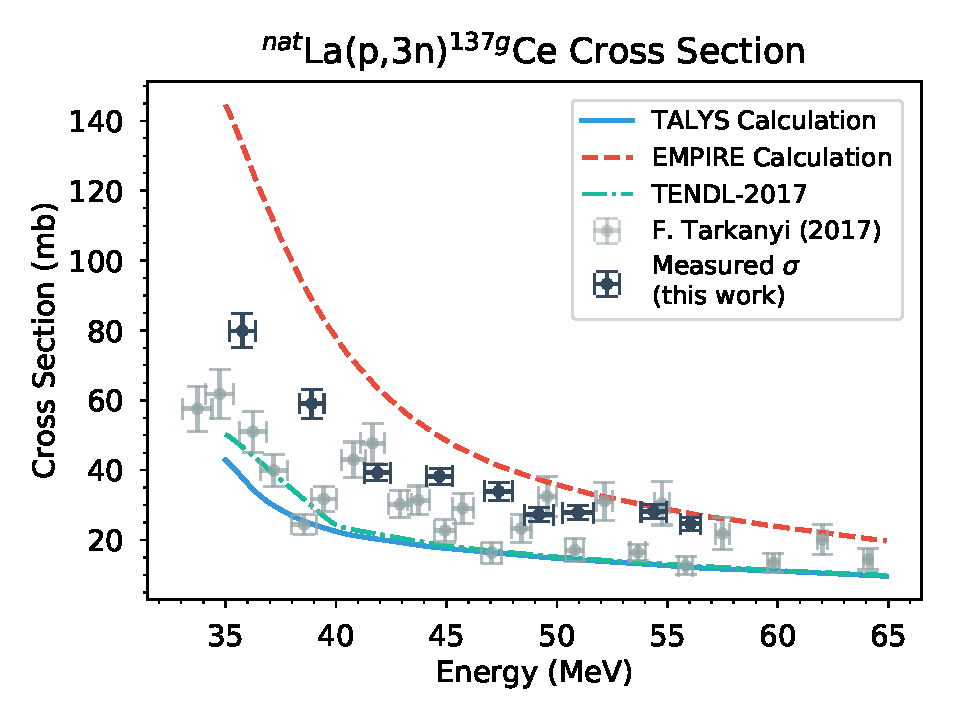
\includegraphics[width=0.32\linewidth]{cross_sections/137CEg.pdf}
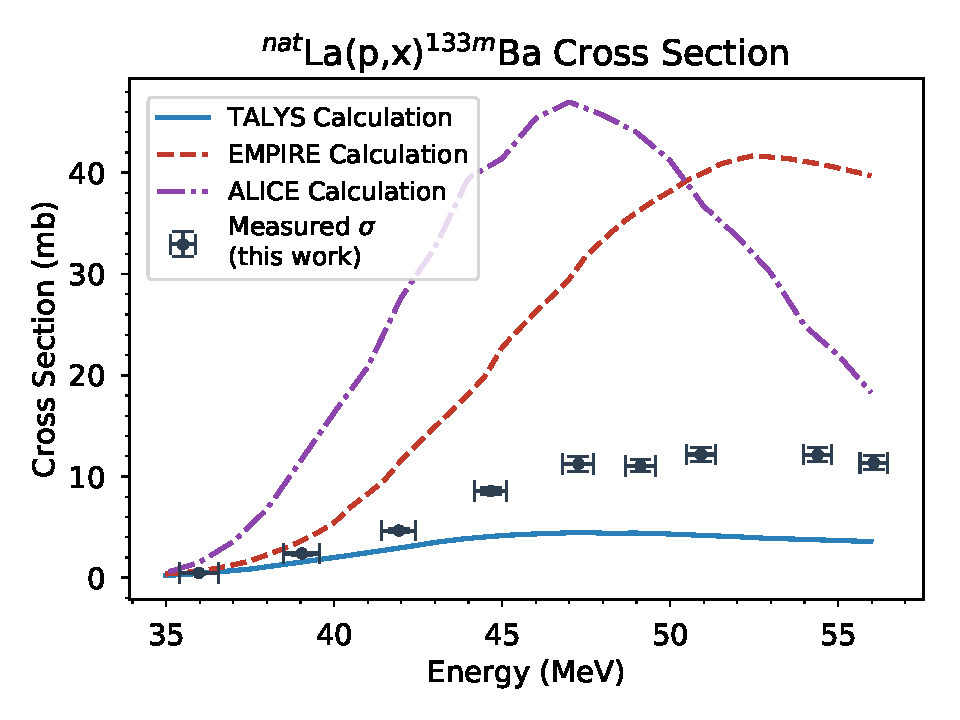
\includegraphics[width=0.32\linewidth]{cross_sections/133BAm.pdf}
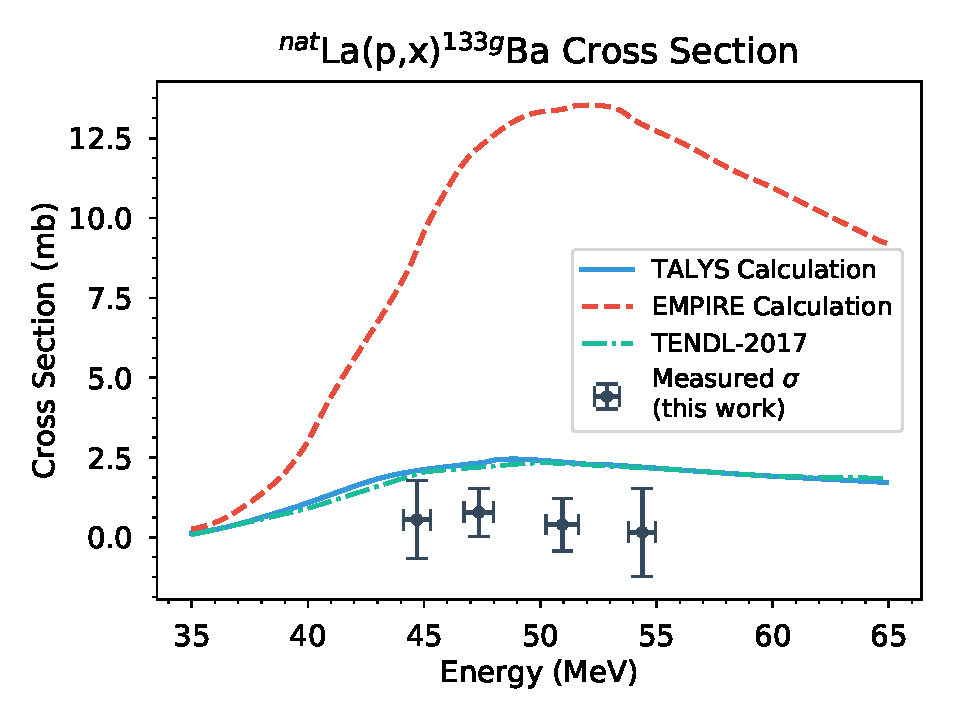
\includegraphics[width=0.32\linewidth]{cross_sections/133BAg.pdf}\\
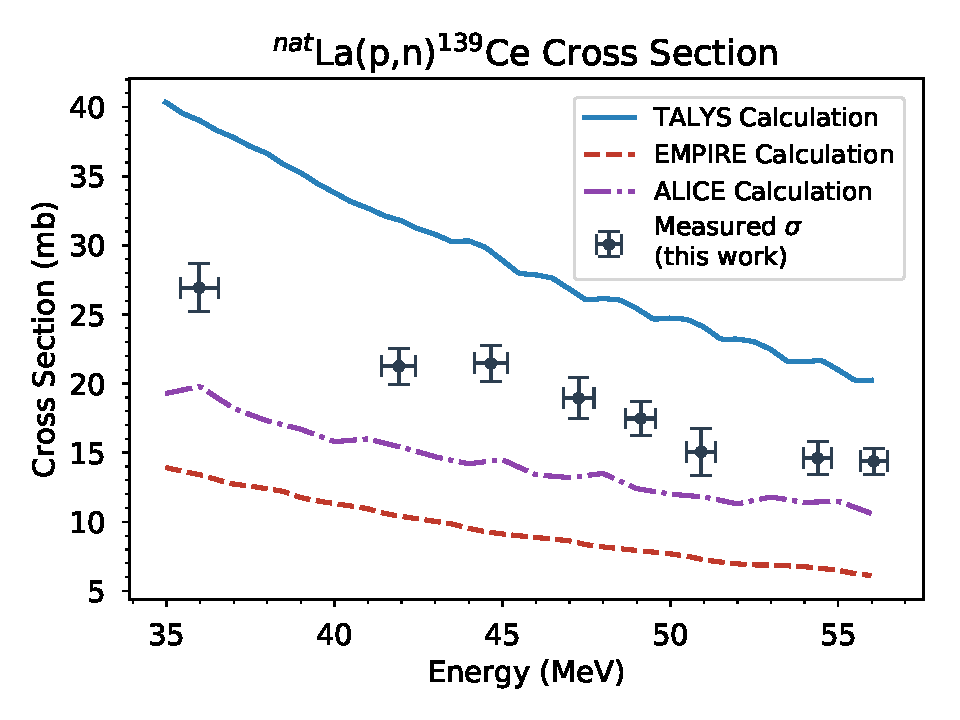
\includegraphics[width=0.32\linewidth]{cross_sections/139CE.pdf}
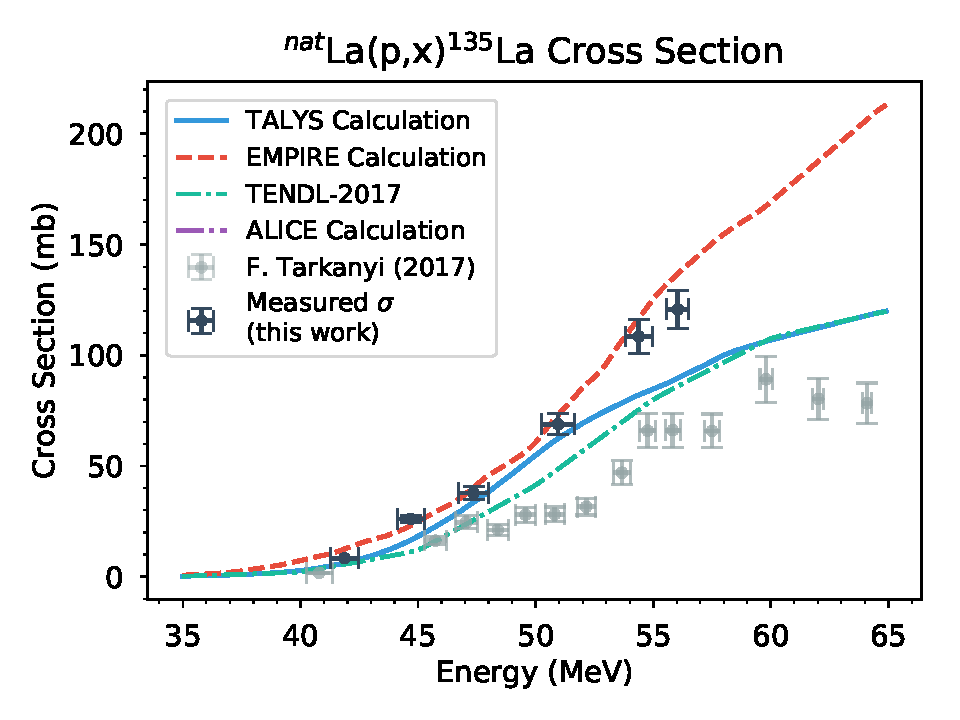
\includegraphics[width=0.32\linewidth]{cross_sections/135LA.pdf}
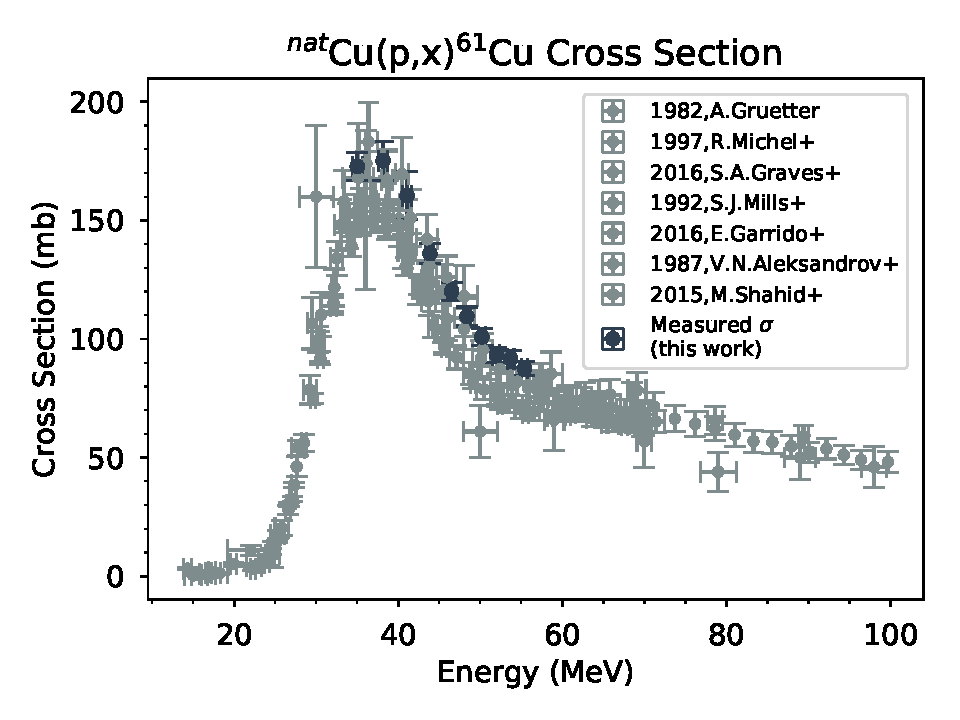
\includegraphics[width=0.32\linewidth]{cross_sections/61CU.pdf}
\caption{Measured excitation functions in $^{nat}$La (first 8) and $^{nat}$Cu (lower right).  TALYS and EMPIRE calculations shown in solid blue and dashed red, respectively.}
\end{figure}

%----------------------------------------------------------------------------
\begin{columns}[t,totalwidth=\twocolwid] % Split up the two columns wide column again
\begin{column}{\onecolwid} % The first column within column 2 (column 2.1)
%----------------------------------------------------------------------------
%----------------------------------------------------------------------------
\begin{block}{Methodology}
\small{\hspace*{50pt}The cross section for a given incident beam energy can be calculated using the activation method by the following equation

\begin{equation}
\sigma =  A_0[I_p \rho \Delta r (1-e^{-\lambda t_i})]^{-1}
\label{eq:xs_calc}
\end{equation}

where $A_0$ is the activity of a given reaction product at the end of irradiation, $I_p$ is the proton beam current, $\rho \Delta r$ is the areal number density and the factor $(1-e^{-\lambda t_i})$ is the ratio of induced activity to the saturation activity, where $\lambda$ is the decay constant for a given reaction product and $t_i$ is the total irradiation time. 

\hspace*{50pt}The activity $A_0$ is determined by collecting a spectrum of $\gamma$-ray emissions. If a $\gamma$ spectrum is counted for a measurement time $t_m$, beginning some amount of time $t_c$ after the proton beam was shut off, then the end-of-beam activity measured in a photo-peak having $N_c$ counts will be

\begin{equation}
A_0 = \frac{\lambda N_c}{(1-e^{-\lambda t_m})e^{-\lambda t_c}I_{\gamma}\epsilon}
\label{eq:activity}
\end{equation}

where $I_{\gamma}$ is the $\gamma$ emission fraction per decay and $\epsilon$ is the detector efficiency at that particular photo-peak energy.
}

\end{block}
%----------------------------------------------------------------------------
\end{column} % End of column 2.1
\begin{column}{\onecolwid} % The second column within column 2 (column 2.2)
%----------------------------------------------------------------------------
%----------------------------------------------------------------------------
\begin{block}{Energy Assignments}

\small{\hspace*{50pt}The energy centroids (and $\sigma_E$) were first estimated using the MCNP output, however there was a large spread in the apparent beam current values seen by each monitor reaction channel.  This was indicative of incorrect characterization of the proton energy spectra incident on each monitor foil.  In order to correct for this, the areal density of the degrader foils and the incident proton beam energy were treated as free parameters, and were varied in order to find the energy assignments yielding the smallest variance in the beam current.}

\begin{figure}
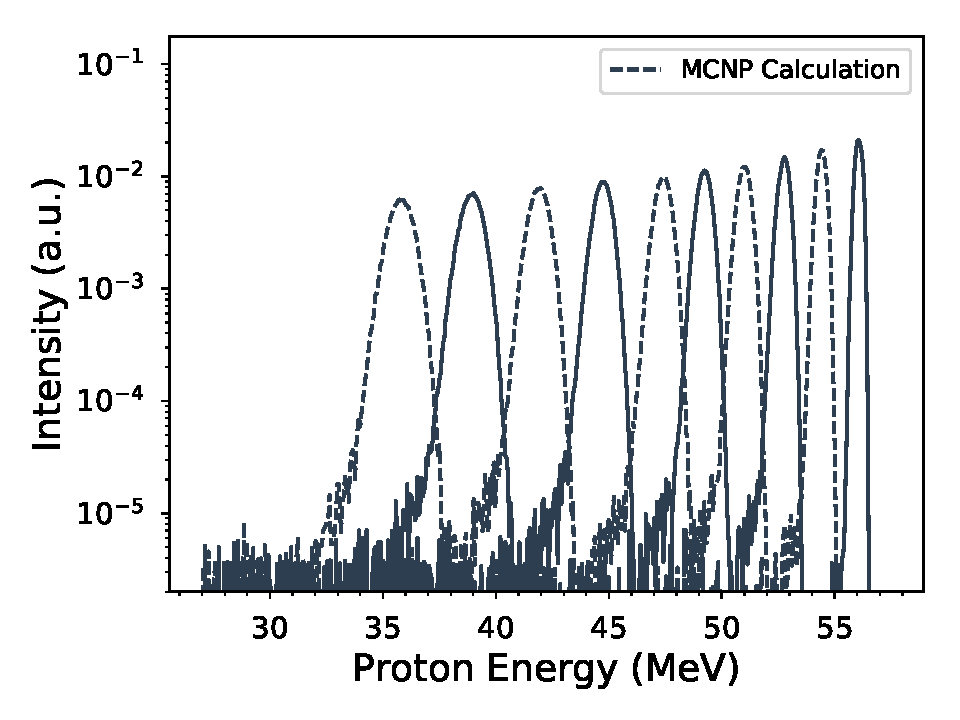
\includegraphics[width=0.48\linewidth]{monitors/La_mcnp_spectrum.pdf}
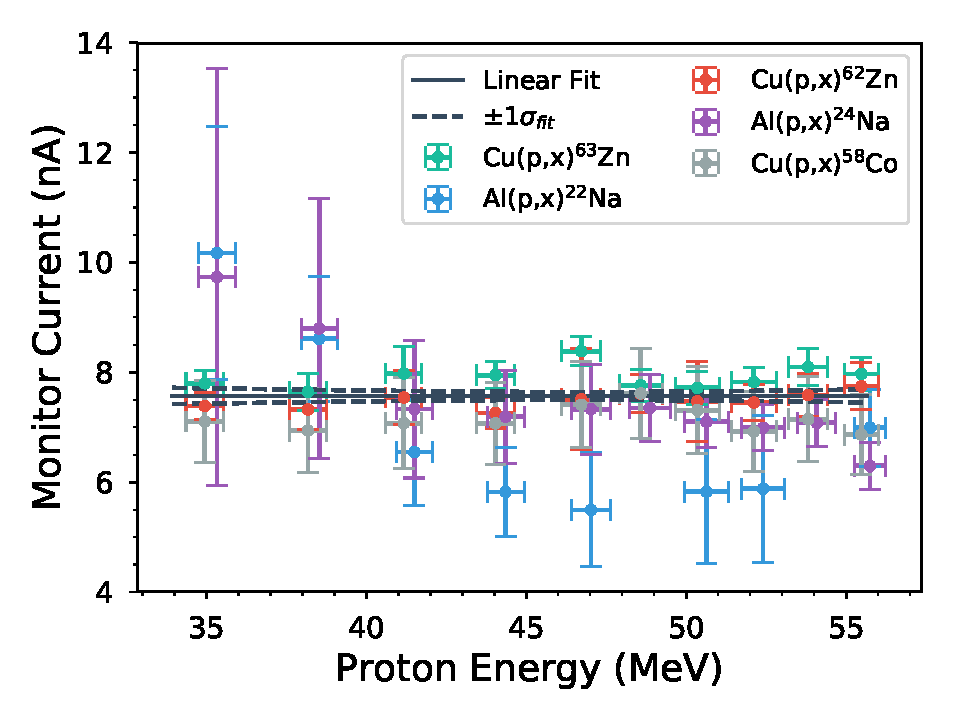
\includegraphics[width=0.48\linewidth]{monitors/current_norm_mcnp.pdf}
\caption{Left: Plot of the proton energy spectra for each lanthanum foil in the target stack. Right: Plot of the beam current measured by each monitor foil reaction, with a linear fit (and $\pm 1 \sigma$) plotted in black.}
\end{figure}

\end{block}
%----------------------------------------------------------------------------
\end{column} % End of column 2.2
\end{columns} % End of the split of column 2
\end{column} % End of the second column
\begin{column}{\sepwid}\end{column} % Empty spacer column
\begin{column}{\onecolwid} % The third column

%----------------------------------------------------------------------------
%   RIGHT
%----------------------------------------------------------------------------
\begin{block}{Results and Discussion}
\small{\hspace*{50pt}Figure 3. shows the measured cross sections for various $^{nat}$La(p,x) reactions, using a 57 MeV proton beam at the LBNL 88" cyclotron and a stacked foil target.  We also compared these measurements with the outputs of the TALYS and EMPIRE nuclear reaction modelling codes, using default parameters.  In most cases neither code accurately predicted the magnitude of the cross sections, but TALYS consistently underpredicted the energy of the peak in the cross section, whereas the EMPIRE predictions agreed with the shape of the measured cross sections quite well.  This primarily speaks to the fidelity of the pre-equillibrium models used by the respective codes: the hybrid Monte Carlo simulation model (EMPIRE) typically produced better predictions than the exiton model (TALYS).

\hspace*{50pt}Particular attention to detail was taken measuring the production of $^{134}$Ce, an isotope with applications as a positron emitting analogue of the medically relevant $^{225}$Ac isotope.  The results of this study show that a higher energy proton beam will be required to produce $^{134}$Ce using this reaction than was previously calculated.  The highest energy proton beam availible at the LBNL 88" cyclotron (57 MeV) produces an unacceptable activity of other Cerium isotopes, which will act as impurities in a medical study.  A proton beam of at least 70 MeV will be required to produce significant activities of $^{134}$Ce without contaminants.

}

\end{block}
%----------------------------------------------------------------------------
%   REFERENCES
%----------------------------------------------------------------------------
\begin{block}{References}
\nocite{*} % Insert publications even if they are not cited in the poster
\small{\bibliographystyle{unsrt}
\bibliography{LaCe.bib}}
\end{block}
%----------------------------------------------------------------------------
%   ACKNOWLEDGEMENTS
%----------------------------------------------------------------------------
\begin{block}{Acknowledgements}
\small{\rmfamily{\hspace*{50pt}We wish to acknowledge our thanks to the operators of the 88" cyclotron: Brien Ninemire, Nick Brickner, Tom Gimpel and Scott Small for their efforts in setting a new "high-water mark" for the maximum proton energy extracted from the machine.  This work has been performed under the auspices of the U.S. Department of Energy by Lawrence Berkeley National Laboratory under contract No. LAB16-1588 NSD.}} \\
\end{block}
%----------------------------------------------------------------------------
%----------------------------------------------------------------------------

\begin{itemize}
\item Email: \href{mailto:jmorrell@berkeley.edu}{jmorrell@berkeley.edu}
\end{itemize}

%----------------------------------------------------------------------------
\end{column} % End of the third column
\end{columns} % End of all the columns in the poster
\end{frame} % End of the enclosing frame
\end{document}
              
            